%!TEX program = lualatex
\documentclass[14pt]{constructor-thesis}

\usepackage[backend=bibtex]{biblatex}
\usepackage{tikz}
\usepackage{import}
\usepackage[mathscr]{euscript}
\usepackage{amsmath,amsthm,amssymb,latexsym,amsfonts}
\usepackage{thmtools}
\usepackage{lipsum}
\usepackage{soul}
\usepackage{amsmath,amssymb}
\usepackage{parskip}
\usepackage{graphicx}
\usepackage{mathtools}
\usepackage[usestackEOL]{stackengine}
\usepackage{tocloft}
\usepackage{xcolor}
\usepackage{hyperref}
\usepackage{tikz}
% \usepackage{pdfcomment}
% \usepackage{blindtext}
% \usepackage{todonotes}
\usepackage{hyphsubst}
\usepackage{bookmark}
\usepackage{pgfplots}
\usepackage{tikzsymbols}
\usepackage{cancel}
\usepackage{enumerate}
% \usepackage{wrapfig}
% \usepackage{graphicx}
\usepackage{extarrows}
\usepackage[bottom]{footmisc}
\usepackage[many]{tcolorbox}
\usepackage{syntax}
% \usepackage[table]{xcolor}
\addbibresource{thesis.bib}

\theoremstyle{definition}
\newtheorem{theorem}{Theorem}
\newtheorem{lemma}{Lemma}
\newtheorem{definition}{Definition}

\newcommand{\pathstart}[1]{(#1)}
\newcommand{\pathhop}[3]{#1 \texttt{-[} #2 \texttt{]-} (#3)}

\newcommand{\patternstart}[1]{(#1)}
\newcommand{\patternhop}[3]{#1 \texttt{-[[} #2 \texttt{]]-} (#3)}

\newcommand{\todo}[1]{
  \begin{tcolorbox}[colframe=red!75!black,colback=red!5!white,arc=0pt,fonttitle=\bfseries]
  \textbf{TODO:} #1
  \end{tcolorbox}
}

% \feetbelowfloat

\begin{document}
% Год, город, название университета и факультета предопределены,
% но можно и поменять.
% Если англоязычная титульная страница не нужна, то ее можно просто удалить.
\filltitle{en}{
  chair              = {Bachelor of Science \\ Computer Science},
  title              = {Mechanizing semantics of graph query languages in Coq},
  author             = {Semen Panenkov},
  supervisorPosition = {Prof.},
  supervisor         = {Anton Podkopaev},
  reviewerPosition   = {},
  reviewer           = {},
  chairHeadPosition  = {Dr.},
  chairHead          = {Stanislav Protasov},
}
\maketitle
\tableofcontents
% У введения нет номера главы
\section*{Introduction}

Databases have come a long way since their inception, and today we have a plethora of database types available, each designed to serve a particular use-case~\cite{database-types}. One of the more recent types to gain popularity are graph databases.

As the name suggests, graph databases represent data using graphs. While the idea of representing data with graphs is not new with solutions developed as early as the mid-1960s, the first enterprise-ready ACID-compliant transactional database only emerged in 2007 with the release of Neo4j~\cite{enwiki:1146498781}. Since then, many graph databases such as Amazone Neptune, RedisGraph and NebulaGraph have sprung up~\cite{enwiki:1146498781}, with successful applications in various fields including recommendation services, fraud detection in finance~\cite{neo4j:use-cases} and even investigations of corruption schemes~\cite{icij:offshoreleaks}.

% However, despite the growing popularity of graph databases, the lack of a standardized query language poses significant challenges to their wider adoption. The graph database community has developed Graph Query Language (GQL) to address this need. Nevertheless, standardizing GQL is challenging due to its complexity and constant expansion, and can result in errors and ambiguities even after thorough reviews~\cite{cpp-std-verified}. Furthermore, given the declarative nature of GQL, the database needs to determine how to fetch the data described in the query, leading to a greater number of possible implementations. This even poses into question the very existence of a realistic implementation.

However, unlike relational databases world with its SQL, there is no standardized language for these systems. In response, the graph database community has developed Graph Query Language (GQL) which is currently being standardized. Standardization is essential for a query language because it simplifies the databases development process and makes it easier to create applications that can work across different graph database systems. With a standardized language like GQL, developers can write queries in a familiar syntax that can be easily understood and executed by different graph databases, promoting interoperability and making it easier to work with data stored in different systems.

Nevertheless, standardizing GQL is challenging due to its complexity and constant expansion, and can result in errors and ambiguities even after thorough reviews as the experience with another well-known standardized language has shown~\cite{cpp-std-verified}.

There has been an attempt to mathematically formalize the standard~\cite{GQL-formalized-on-paper} which we used as a reference, however, this attempt is still pen-and-paper and, as a result, is prone to errors. In fact, we have identified some errors in the aforementioned paper.


Furthermore, given the declarative nature of GQL, the database needs to determine how to fetch the data described in the query, leading to a greater number of possible implementations. The very existence of a realistic implementation can be questioned in this case.

In fact, graph databases translate a query into an intermediate representation called \textbf{execution plan}, which is just a chain of operations that need to be performed in order to evaluate the query. These operations inspect the graph and produce intermediate results that are later transformed by subsequent operations. This solution draws inspiration from relational databases world, where such approach has proven to be successful. Moreover, the translation process itself is complex and contains a lot of subtle details which are easy to overlook.

% TODO: Describe the errors in the paper.

% In fact, graph databases translate a query into an intermediate representation called \textbf{execution plan}, which is just a sequence of operations that need to be performed in order to evaluate the query. These operations inspect the graph and produce intermediate results that are later transformed by subsequent operations. This solution draws inspiration from relational databases world, where such approach has proven to be successful.

% However, this still leaves a lot of space to the implementators of the standard. For example, Neo4j and RedisGraph use different sets of operations and implement them differently. The former divides a query into a large sequence of small and simple operations while the latter covers with one complex operation the bigger part of a query but its operations are heavily optimized using linear algebra. The situation is further complicated by the fact that the translation process itself is complex and contains a lot of subtle details.

To address these challenges, we develop a mechanized specification of GQL and the key details of query evaluation. Specifically, we aim to mechanize the semantics of the subset of GQL and demonstrate the correctness of the way that Neo4j and RedisGraph, our reference databases, translate queries to execution plans. To achieve this goal, we use the Coq proof assistant, a programming language that allows us to write and reason about programs with greater rigor and confidence. The key point is that proofs written in Coq are machine-checkable. By providing a more robust approach to checking the correctness of the ecosystem around GQL, this work has the potential to contribute significantly to the wider adoption of graph databases.

There has been a successful attempt to mechanize a subset of the SQL standard~\cite{sql-in-coq} and even write a verified relational database in Coq~\cite{rdbms-in-coq}. Their experience has shown that though many challenges remain, building fully-verified systems software in Coq is within reach.

% It allows to define mechanised, executable specifications whose correctness is machine-checkable.

% Competing graph databases typically use some dialect of the Cypher query language, much like how different relational databases use SQL. However, unlike SQL, there is no agreed-upon standard for Cypher. To address this, the graph database community developed Graph Query Language (or GQL), which is currently being standardized by ISO.

% This standard, like any other ISO standard, is just an informal human-readable text. Experience with other complex stardardized languages like C++ has shown that, despite the fact that such standards undergo a thorough review, they can still left some parts unspecified~\cite{cpp-std-verified} and even contain errors (citation needed about C++ memory model).

% Even if we concentrated all our efforts on correcting the current version of the standard, it would be impossible to maintain due to the fact that GQL is constantly being expanded.

% Moreover, proving that the standard is realistic and practical requires to actually implement the standard, i. e. to provide an evaluator of the GQL queries which complies with the standard.

% The situation is further complicated by the fact that GQL is a declarative language, meaning queries only describe what data is required, and the database has to figure out how to fetch it. This increases the number of possible implementations and may require us to introduce additional constructions to be able to evaluate the query. 

% In fact, graph databases translate a query into an intermediate representation called \textbf{execution plan}, which is just a sequence of operations that need to be performed in order to evaluate the query. These operations inspect the graph and produce intermediate results that are later transformed by subsequent operations. This solution draws inspiration from relational databases world, where such approach has proven to be successful.

% However, this still leaves a lot of space to the implementators of the standard. For example, Neo4j and RedisGraph use different sets of operations and implement them differently. The former divides a query into a large sequence of small and simple operations while the latter covers with one complex operation the bigger part of a query but its operations are heavily optimized using linear algebra.

% Moreover, the translation process itself is complex and contains a lot of subtle details.

% All of these notes imply that we need a more robust approach to check the correctness of all the parts that constitute the ecosystem around the currenly developed standard than just being careful.

% This is why we have decided to formalize the GQL standard and prove that the key details of the query evaluation are correct. Specifically, our aim is to demonstrate the correctness of the way that our reference databases, Neo4j and RedisGraph, translate queries to execution plans.

% To achieve that goal, we have chosen the Coq proof assistant which is basically a programming language that allows for writing and reasoning about programs.

\section{Goals and objectives}

Let us state our goal again. We want to mechanize the core subset of the GQL standard and its two main implementations in Coq.

To achieve this goal, we have set the following objectives:
\begin{itemize}
  \item \textbf{Mechanize the specification of the core subset of the GQL standard}:
  
  First, we want to write a specification for some subset of GQL. We want to define it the way that allows us to abstract from the implementation details of the query evaluation and reason about high-level properties.

  \item \textbf{Mechanize the specification of the execution plan}:
  
  Secondly, we want to specify some key operations of execution plans that are necessary to evaluate our queries. From this specification we want the same properties as from the specification of GQL.

  \item \textbf{Implement and prove the correctness of the translation of the queries}:
  
  The next objective is to define the translation from queries to execution plans and show that it is correct. Correctness in this case means that, according to the specification of the execution plan, the evaluation of translated queries satisfies the specification of GQL.

  \item \textbf{Provide an example implementation of the execution plan evaluation}:
  
  It is also very important to implement those operations to prove that the specification we provided is realistic. We don't aim for a performant or a production-ready implementation, however, we want to capture the way RedisGraph optimizes its operations using linear algebra.

\end{itemize}

\section{Related work}

In this section we describe the basics of GQL and graph databases. For formal definitions we refer the reader to section~\ref{sec:technical-details}. We assume some familiarity with SQL and relational databases.

\subsection{Property Graphs}
\label{section:intro-property-graphs}

Graph databases use so-called property graphs as an underlying data model. \textbf{A property graph} is a directed multigraph where each node\footnote{In the rest of the text we use words ``node'' and ``vertex'' interchangeably} or edge can store a possibly empty set of property-value pairs. To distinguish nodes and edges, each node and edge has a unique identifier\footnote{Even though any two vertex identifiers must differ as well as any two edge identifiers, sets of vertex and edge identifiers can overlap. They are considered to belong to different namespaces.}. In addition, labels can be added to nodes and edges to indicate their meaning.

\begin{figure}[b]
  \centering
  
  \import{img/}{property-graph.tex}

  \caption{Example property graph}
  \label{fig:property-graph}
\end{figure}

For instance, in figure~\ref{fig:property-graph} there are two nodes labelled ``Person'' and ``Company'' with identifiers 0 and 1, respectively. The company has a property ``name'' with a value of ``JB'', and there is an edge from the person to the company labelled ``WORKS\_FOR'' with id of 0. This edge also has a property ``since'' with a value of ``2022''.

\subsection{Binding tables}
\label{section:intro-binding-tables}

The result of a GQL query is represented with a so-called binding table which is analogous to the relation from SQL. Binding tables are also used to represent the intermidiate results during the query evaluation.

Basically, \textbf{a binding table} is a list of records. Each \textbf{record} is a tuple of values with named fields. \textbf{The domain of a record} is a set of all used names. \textbf{The type of a record} is a tuple with named fields of types of values under these names. A particular name-type pair is called \textbf{an attribute}. All the records in a table must have the same type, i.e. their domains must be the same and types of values under the same name must also match.

Because of the fact that all the records in any table have the same type, we can define \textbf{the type of a table} as the type of any of its records. An attribute of a record is also an attribute of the table.

\begin{table}
  \centering
  
  \begin{tabular}{ |p{3cm}|p{3cm}|p{3cm}|  }
    \hline
    \texttt{v : vertex} & \texttt{e : edge} & \texttt{u : vertex} \\
    \hline
    0 & 0 & 1 \\
    2 & 1 & 1 \\
    \hline
  \end{tabular}

  \caption{Example binding table}
  \label{tab:example-binding-table}
\end{table}

For example, in Table~\ref{tab:example-binding-table} there are two records and three attributes: \texttt{v : vertex}, \texttt{e : edge}, and \texttt{u : vertex}. 


\subsection{GQL queries syntax and semantics}
\label{section:intro-GQL}

GQL queries consist of clauses, keywords and expressions (like predicates and functions) many of which will be familiar to the users of SQL.


The following example query consists of three clauses:
\begin{verbatim}
MATCH (p:Person)-[e:WORKS_FOR]->(c:Company {"name": "JB"})
WHERE e.since >= 2020
RETURN *
\end{verbatim}

The first one is the \texttt{MATCH}-clause which allows to specify \textbf{a path pattern}. The result of this clause is a table where entries represent all the paths that match the pattern. The second clause is the \texttt{WHERE}-clause which allows to filter the records based on some predicate. And the last clause just says that we want to retrieve everything.

Let's dive deeply into the syntax of path patterns:
\begin{verbatim}
(p:Person)-[e:WORKS_FOR]->(c:Company {"name": "JB"})
\end{verbatim}

Here \verb+(p:Person)+ and \verb+(c:Company {"name": "JB"})+ are \textbf{vertex patterns} while \verb+-[e:WORKS_FOR]->+ is \textbf{an edge pattern}. \texttt{p}, \texttt{e}, \texttt{c} are vertex and edge pattern names. They are used to refer to the corresponding graph objects in the rest of the query. \texttt{Person} and \texttt{Company} are vertex labels. \texttt{WORKS\_FOR} is an edge label. \texttt{"name": "JB"} is \textbf{a property pattern}. It says that the company must have a property ``name'' with a value of ``JB''.

\begin{table}[b]
  \centering
  
  \begin{tabular}{ |p{3cm}|p{3cm}|p{3cm}|  }
    \hline
    \texttt{p : vertex} & \texttt{e : edge} & \texttt{c : vertex} \\
    \hline
    0 & 0 & 1 \\
    \hline
  \end{tabular}

  \caption{The result of the example query}
  \label{tab:example-query-binding-table}
\end{table}

Names of edge patterns are distinct and must differ from names of vertex patterns. However, names of vertex patterns can repeat. This can be used, for example, to look for cycles in the graph.

Names, labels and property patterns are optional. If a name is not specified, the matching graph objects are not listed in the result. For example, \texttt{()} is a completely valid vertex pattern.

The syntax \texttt{-[]->} says that the edge is directed from left to right, from the person to the company. We can also use \texttt{<-[]-} to match the edges in the reversed direction. And \texttt{-[]-} to say that the direction of the edge does not matter.

From the formal point of view, these paths are not simple paths, i. e. they are actually walks. You can think of them as alternating sequences of vertex and edge identifiers which must have the same length as the path pattern and each vertex or edge identifier must satisfy the restrictions imposed by the vertex or edge pattern on the same position.

For example, the paths that satisfy the example path pattern have the following form: $\pathhop{\pathstart{v_1}}{e}{v_2}$. Where $v_1$ must satisfy the vertex pattern \verb+(p:Person)+, $e$ must satisfy the edge pattern \verb+-[e:WORKS_FOR]->+ and $v_2$ must satisfy the vertex pattern \verb+(c:Company {"name": "JB"})+.

In the \texttt{WHERE}-clause the predicate \verb+e.since >= 2020+ says that the edge must have a property ``since'' with an integer value greater than or equal to 2020.

% TODO: grammar for the subset of GQL

If we run the example query on the example graph from Figure~\ref{fig:property-graph}, we will get binding table~\ref{tab:example-query-binding-table}. This is because there is only one path in the graph that matches the pattern: $\pathhop{\pathstart{0}}{0}{1}$ (node 0 has the label \texttt{Person}, node 1 has a label \texttt{Company} and edge 0 has a label \texttt{WORKS\_FOR} and a property ``name'' with a value of ``JB''). Edge 0 also has a property ``since'' with a value of 2022 which is greater than 2020. So the predicate is true and the record is included in the result.

\subsection{Execution plans}

As you could see, GQL is a declarative language, meaning queries only describe what data is required, and the database has to figure out how to fetch it.

Like relational databases, graph databases translate a query into an intermediate representation called \textbf{an execution plan}, which is just a sequence of operations that need to be performed in order to evaluate the query. These operations inspect the graph and produce intermediate binding tables that are later transformed by subsequent operations.

Moreover, the optimization step of the query evaluation is usually performed on the execution plan of the query.

Our reference databases, Neo4j and RedisGraph, use different sets of operations to evaluate queries. However, the general idea is the same.

\begin{figure}
  

\tikzset{every picture/.style={line width=0.75pt}} %set default line width to 0.75pt        

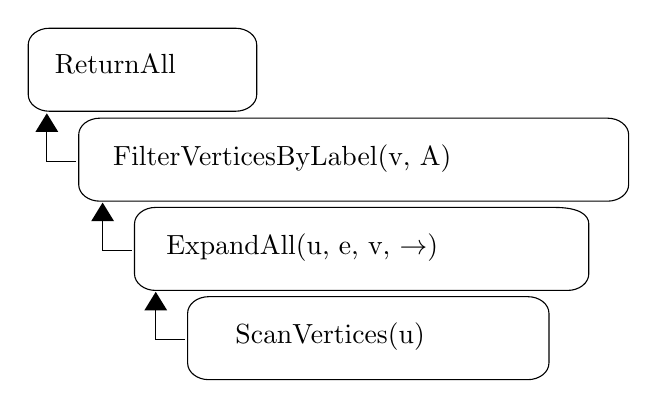
\begin{tikzpicture}[x=0.75pt,y=0.75pt,yscale=-1,xscale=1.28]
%uncomment if require: \path (0,531); %set diagram left start at 0, and has height of 531

%Rounded Rect [id:dp9370573454267987] 
\draw   (111,40) .. controls (111,35.58) and (114.58,32) .. (119,32) -- (189,32) .. controls (193.42,32) and (197,35.58) .. (197,40) -- (197,64) .. controls (197,68.42) and (193.42,72) .. (189,72) -- (119,72) .. controls (114.58,72) and (111,68.42) .. (111,64) -- cycle ;

%Rounded Rect [id:dp6856967461478435] 
\draw   (130,83.33) .. controls (130,78.91) and (133.58,75.33) .. (138,75.33) -- (329,75.33) .. controls (333.42,75.33) and (337,78.91) .. (337,83.33) -- (337,107.33) .. controls (337,111.75) and (333.42,115.33) .. (329,115.33) -- (138,115.33) .. controls (133.58,115.33) and (130,111.75) .. (130,107.33) -- cycle ;
%Straight Lines [id:da3265514824492094] 
\draw    (129,96) -- (118,96) -- (118,76) ;
\draw [shift={(118,73)}, rotate = 90] [fill={rgb, 255:red, 0; green, 0; blue, 0 }  ][line width=0.08]  [draw opacity=0] (8.93,-4.29) -- (0,0) -- (8.93,4.29) -- cycle    ;
%Rounded Rect [id:dp4438884800021361] 
\draw   (151,126.33) .. controls (151,121.91) and (154.58,118.33) .. (159,118.33) -- (339 - 30,118.33) .. controls (343.42 - 25,118.33) and (347-25,121.91) .. (347 - 25,126.33) -- (347 - 25,150.33) .. controls (347 - 25,154.75) and (343.42 - 25,158.33) .. (339 - 25,158.33) -- (159,158.33) .. controls (154.58,158.33) and (151,154.75) .. (151,150.33) -- cycle ;
%Straight Lines [id:da8951131696919742] 
\draw    (150,139) -- (139,139) -- (139,119) ;
\draw [shift={(139,116)}, rotate = 90] [fill={rgb, 255:red, 0; green, 0; blue, 0 }  ][line width=0.08]  [draw opacity=0] (8.93,-4.29) -- (0,0) -- (8.93,4.29) -- cycle    ;
%Rounded Rect [id:dp8868145464168437] 
\draw   (171,169.33) .. controls (171,164.91) and (174.58,161.33) .. (179,161.33) -- (299,161.33) .. controls (303.42,161.33) and (307,164.91) .. (307,169.33) -- (307,193.33) .. controls (307,197.75) and (303.42,201.33) .. (299,201.33) -- (179,201.33) .. controls (174.58,201.33) and (171,197.75) .. (171,193.33) -- cycle ;
%Straight Lines [id:da6792309496243043] 
\draw    (170,182) -- (159,182) -- (159,162) ;
\draw [shift={(159,159)}, rotate = 90] [fill={rgb, 255:red, 0; green, 0; blue, 0 }  ][line width=0.08]  [draw opacity=0] (8.93,-4.29) -- (0,0) -- (8.93,4.29) -- cycle    ;

% Text Node
\draw (120,43.5) node [anchor=north west][inner sep=0.75pt]   [align=left] {ReturnAll};
% Text Node
\draw (142,86.83) node [anchor=north west][inner sep=0.75pt]   [align=left] {FilterVerticesByLabel(v, A)};
% Text Node
\draw (162,129.83) node [anchor=north west][inner sep=0.75pt]   [align=left] {ExpandAll(u, e, v, $\rightarrow$)};
% Text Node
\draw (188,172.83) node [anchor=north west][inner sep=0.75pt]   [align=left] {ScanVertices(u)};


\end{tikzpicture}

  \caption{The Neo4j execution plan for the example path pattern}
  \label{fig:intro-execution-plan}
\end{figure}

Consider an example query with a pattern \texttt{(u)-[e]->(v:A)}. Figure~\ref{fig:intro-execution-plan} shows the execution plan that Neo4j might build for it. The evaluation of the query starts from fetching all vertices from the graph and adding them to the resulting table under name $u$. Then, for each vertex $u$ in the table, Neo4j fetches all outgoing edges from $u$ and adds them to the table under name $e$ alongside with the destination nodes of these edges under name $v$. After that, for each vertex under name $v$ it checks that this vertex has label $A$ and discards the records which do not satisfy the criteria. Finally, it returns the resulting table cleaning up all the auxilliary information but there is none in this case.

\section{The specification of GQL semantics and key details of query evaluation}
\label{sec:technical-details}

In this section we describe how we have achieved each of the stated objectives. We show the concrete definitions and theorems that we have proved as well as the ideas behind them.

\subsection{The specification of the core subset of GQL}

We start with the description of the core subset of GQL. First, we formally describe the concrete syntax of the subset. Then we formally specify its abstract syntax and semantics.

We decided to provide the specification via denotational semantics. In other words, we describe which properties the resulting binding table should satisfy. This approach is very convenient for us because it allows us to write a specification in a very high-level way and treat the actual implementation of the specification later. However, this approach requires us to show that the specification is complete in some sense. We do this by proving that any two implementations of the specification are equivalent, i. e. for the same queries they produce same results.

Our specification closely follows the aforementioned formalization~\cite{GQL-formalized-on-paper}. However, we have introduced some new concepts and changed some definitions to make them more convenient for us. For example, we introduced the notion of types that allowed us to state well-formedness conditions in a simple way. We also introduced implicit names to model the query normalization which our reference databases perform. Moreover, we introduced matching modes to control which names occur in the resulting table. This allowed us to reason about the auxilliary information that graph databases use during query evaluation.

\subsubsection{The concrete syntax of the subset}
\label{sec:GQL-syntax}

\begin{figure}
  \newcommand*{\myfont}{\fontfamily{lmss}\selectfont}
  \newcommand*{\myfonttt}{\fontfamily{lmtt}\selectfont}
  \renewcommand{\syntleft}{\myfont\color{black} }
  \renewcommand{\syntright}{}
  \renewcommand{\litleft}{\myfonttt\bfseries\color{red}}
  \renewcommand{\litright}{}
  \setlength{\grammarparsep}{5pt plus 1pt minus 1pt} % increase separation between rules
  \setlength{\grammarindent}{10em} % increase separation between LHS/RHS 
  \begin{tcolorbox}[colframe=gray!50!white,colback=gray!5!white,arc=0pt]
    \begin{grammar}

      <path-pattern> ::= <vertex-pattern> (<edge-pattern> <vertex-pattern>)*

      <vertex-pattern> ::= `(' <pattern-body> `)'

      <edge-pattern> ::= `-[' <pattern-body> `]->'
      \alt `<-[' <pattern-body> `]-'
      \alt `-[' <pattern-body> `]-'

      <pattern-body> ::= <name>? <label-pattern>? <properties-pattern>?

      <label-pattern> ::= `:' <label>

      <properties-pattern> ::= `\{' <property> (`,' <property>)* `\}'

      <property> ::= <key> `:' <value>

      <query> ::= `MATCH' <path-pattern> \\ `RETURN *'
      
    \end{grammar}
  \end{tcolorbox}
  \caption{The grammar for concrete syntax of the core subset of GQL}
  \label{fig:GQL-grammar}
\end{figure}

The concrete syntax of the core subset of GQL is given by the grammar in Figure~\ref{fig:GQL-grammar}. We use the following conventions:
\begin{itemize}
  \item \textbf{Non-terminals} are written in black normal font.
  \item \textbf{Terminals} are written in red type-writer font.
\end{itemize}

We have chosen to only formalize the \texttt{MATCH}-clause in its simplest but still meaningful form. The semantics of this subset has been informally discussed in the introduction.

In the next sections, we will define the abstract syntax of this subset, its semantics and underlying mathematical objects.

\subsubsection{Values}
\label{sec:GQL-values}

\begin{definition}
  We have the following \textbf{types} of \textbf{values} in our specification:
  \begin{itemize}
    \item \textbf{Graph object types.} Values of these types are vertex and edge identifiers. We denote the type of vertex identifiers by $\mathtt{vertex}$ and the type of edge identifiers by $\mathtt{edge}$.
    \item \textbf{Base types.} Values of these types are floating point numbers, integers and strings. We denote these types by $\mathtt{float}$, $\mathtt{int}$ and $\mathtt{string}$, respectively.
    \item \textbf{Boolean type.} Values of this type are either \texttt{true}, \texttt{false} or \texttt{unknown}. We denote this type by $\mathtt{bool}$.
  \end{itemize}
\end{definition}

You might be confused by the presence of a third value in the boolean type but three-valued logic is a norm in databases world. However, carefully defining the semantics of \texttt{unknown} and its interaction with values of other types is out of the scope of this project. We will only use graph object types. Other types are introduced for the sake of building examples.

\begin{definition}
  Given the value $v$ we can define the ``type of'' operator: $\mathtt{T}(v)$. It returns the type of the value $v$. For example, if we use ``1'' as an integer, then $\mathtt{T}(1) = \mathtt{int}$.
\end{definition}

\begin{definition}
  We can also define the typing relation for values. It is denoted by $v : t$ and means that the value $v$ has the type $t$. For example, $1 : \mathtt{int}$. Note that $v : t$ is equivalent to $\mathtt{T}(v) = t$.
\end{definition}

\subsubsection{Property graphs}

As has already been said, a property graph is a directed labelled multigraph where each vertex or edge can store a possibly empty set of property-value pairs. In this section we formally define property graphs and their components.

\begin{definition}
  To begin we need to define some auxilliary terms: 
  \begin{itemize}
    \item \textbf{Vertex and edge identifiers} are positive integer numbers, i. e. $\mathbb{N}$.
    \item \textbf{Labels} are simply strings over some finite alphabet $\Sigma$. We denote the set of all labels that can ever be used by $L$, although it is just equal to $\Sigma^*$.
    \item \textbf{Properties} are represented as pairs of keys (plain strings) and values and are denoted by $P$.
  \end{itemize}
\end{definition}

\begin{definition}[Property graphs]
  \label{def:property-graph}
  We have chosen the following formal representation of property graphs:
  \begin{itemize}
    \item \textbf{Vertices and edges} are represented as finite sets of identifiers. We denote a set of vertices and a set of edges by $V$ and $E$, respectively. These sets can contain any numbers, however, we want these sets to be as close to $\{1 \dots |V|\}$ and $\{1 \dots |E|\}$ as possible. It is because we want to use these sets as indices in matrices. This way we can minimize the size of the matrices. Requiring that the sets are exactly of this form is, in practice, impossible if we take into account potential updates and deletions of vertices and edges.
    \item \textbf{Edge ends mapping function} denoted by $\eta$ is a function from $E$ to $V \times V$ which maps an edge to its ends. Note that with this definition all the edges are directed.
    \item \textbf{Labelling functions} are functions $\lambda_V : V \to 2^L$ and $\lambda_E : E \to L$ which map vertices and edges to their labels. Note that we use the powerset of labels for $\lambda_V$ because a vertex can have multiple labels. However, an edge can have one and only one label. The label of an edge is often called its \textit{type}. With this definition, we can say that a node $v$ or an edge $e$ has a label $l$ if $l \in \lambda_V(v)$ or $\lambda_E(e) = l$, respectively.
    \item \textbf{Properties mapping functions} are functions $\phi_V : V \to 2^P$ and $\phi_E : E \to 2^P$ which map vertices and edges to their properties. Note that we use the powerset of properties because a vertex or an edge can have multiple properties. However, we restrict those subsets to be finite.
    \item \textbf{A property graph} $G$ is, thus, a collection of all of those pieces. In other words, $G = (V, E, \eta, \lambda_V, \lambda_E, \phi_V, \phi_E)$.
  \end{itemize}
\end{definition}

For instance, the example graph on Figure~\ref{fig:property-graph} is represented as follows:

\begin{equation*}
  \begin{aligned}[t]
    V &= \{0, 1, 2 \} \\
    E &= \{0, 1, 2 \} \\
    \eta: & \\
          & 0 \mapsto (0, 1) \\
          & 1 \mapsto (0, 2) \\
          & 2 \mapsto (1, 2) \\
    \lambda_V: & \\
          & 0 \mapsto \{\texttt{Person}\} \\
          & 1 \mapsto \{\texttt{Company}\} \\
          & 2 \mapsto \{\texttt{Tech}\} \\
  \end{aligned}
  \qquad
  \begin{aligned}[t]
    \lambda_E: & \\
          & 0 \mapsto \texttt{WORKS\_FOR} \\
          & 1 \mapsto \texttt{LIKES} \\
          & 2 \mapsto \texttt{USES} \\
    \phi_V: & \\
          & 0 \mapsto \varnothing \\
          & 1 \mapsto \{(\texttt{``name''}, \, \texttt{``JB''})\} \\
          & 2 \mapsto \{(\texttt{``name''}, \, \texttt{``Coq''})\} \\
    \phi_E: & \\
          & 0 \mapsto \{(\texttt{``since''}, \, \texttt{2022})\} \\
          & 1 \mapsto  \varnothing \\
          & 2 \mapsto \varnothing
  \end{aligned}
\end{equation*}

\subsubsection{Binding tables}

\begin{definition}
  \textbf{A record} is a \textit{partial} mapping from names to values. We formally define names later.
\end{definition}

With this definition, we can ensure that we can't accidentally map the same name to two different values as opposed to defining a record as a set of pairs of names and values.

Note that we use the word \textit{partial} because we want to have records that don't use all the names. Formally, this means that a record is actually a total mapping from a subset of names.

Also note that with this definition, we can represent records with infinite domains, for example, $r(n) = 0$ for all $n$, although we will never construct such records.

The notation $(n \mapsto v)$ means that the name $n$ is mapped to the value $v$. For example, $(\mathtt{a} \mapsto 1)$ is a record that maps the name $\mathtt{a}$ to the value $1$.

\begin{definition}
  We can \textbf{update} the record $r$ by adding a new name-value pair $(n, v)$. We denote the updated record by $(n \mapsto v; r)$ and formally define it as:
  $$
  (n \mapsto v; r)(n') = \begin{cases}
    v & \text{if } n' = n \\
    r(n') & \text{otherwise}
  \end{cases}
  $$
\end{definition}

With these notations we can easily write down any record with a finite domain: $(n_1 \mapsto v_1; n_2 \mapsto v_2; n_3 \mapsto v_3)$.

\begin{definition}
  \textbf{The type of a record} $r$ is denoted by $T(r)$. $T(r)(n)$ is defined iff $r(n)$ is defined and $T(r)(n) = T(r(n))$.
\end{definition}

That is, the type of a record is a function that maps names to types of values stored under these names in the record. Moreover, we use the same update syntax for the types of records. For example, $T(n_1 \mapsto 1; n_2 \mapsto 2.0) = (n_1 \mapsto \mathtt{int}; n_2 \mapsto \mathtt{float})$.

\begin{definition}
  In the similar to values manner, we can define \textbf{the typing relation for records}:
  $$ r : T \Longleftrightarrow T(r) = T $$
\end{definition}

\begin{definition}
  \textbf{A binding table} is some set of records.
\end{definition}

With this definition, we declare that we don't actually care about the order and number of repetitions of records in the table.

\begin{definition}
  We can define \textbf{the typing relation for binding tables}:
  $$ t : T \Longleftrightarrow \forall r \in t, \, r : T $$
\end{definition}

This definition implies that the binding tables in which records have different types don't have types. Moreover, the type is not unique. For example, empty binding table can have any type, although this is the only example. This will make sense later when we show the specification for some execution plan operations. However, this means that we cannot define ``type of'' operator for all binding tables. Luckily, we will not actually need it.

\subsubsection{Patterns and paths}
\label{sec:GQL-patterns-and-paths}

Recall the example query from section~\ref{section:intro-GQL}. As we discussed in that section, the following part of the query is a path pattern:
\begin{verbatim}
  (p:Person)-[e:WORKS_FOR]->(c:Company {"name": "JB"})
\end{verbatim}

Here \verb+(p:Person)+ and \verb+(c:Company {"name": "JB"})+ are vertex patterns in their concrete syntax while \verb+-[e:WORKS_FOR]->+ is an edge pattern. We have discussed the exact syntax earlier.

% \texttt{p}, \texttt{e}, \texttt{c} are vertex and edge pattern names. They are used to refer to the corresponding graph objects in the rest of the query. \texttt{Person} and \texttt{Company} are vertex labels. \texttt{WORKS\_FOR} is an edge label. \texttt{"name": "JB"} is \textbf{a properties pattern}. It says that the company must have a property ``name'' with a value of ``JB''.

\begin{definition} Mathematically (i.e. in abstract syntax) we define these as follows:
  \begin{itemize}
    \item \textbf{Vertex pattern} $\pi_v$ is an object which has a name $n$, an optional label $l$ and, possibly empty, set of properties $p$. We access them using the following operators similar to the ones we used in definition~\ref{def:property-graph}:
    \begin{itemize}
      \item $\alpha(\pi_v) := n$;
      \item $\lambda(\pi_v) := l$ if $l$ is present, otherwise undefined;
      \item $\phi(\pi_v) := p$ which can be empty.
    \end{itemize}

    \item Analogously, \textbf{edge pattern} $\pi_e$ is an object which has a name $n$, an optional label $l$, possibly empty, set of properties $p$ and a direction $d$. We access them using the following operators:
    \begin{itemize}
      \item $\alpha(\pi_e) := n$;
      \item $\lambda(\pi_e) := l$ if $l$ is present, otherwise undefined;
      \item $\phi(\pi_e) := p$ which can be empty;
      \item $\delta(\pi_e) := d$ where $d$ is either $\rightarrow$, $\leftarrow$ or $\leftrightarrow$.
    \end{itemize}
  \end{itemize}
\end{definition}

% \begin{definition}
%   \textbf{A vertex pattern} is denoted by $(n : l \, \{p_1: v_1, \ldots, p_k: v_k\})$ and \textbf{an edge pattern} is denoted by $\texttt{-[}n : l \; \{p_1: v_1, \ldots, p_k: v_k\}\texttt{]->}$ where $n$ is a name, $l$ is a label, and $p_i$ are property keys and $v_i$ are values. $(p_i, v_i)$ pairs consitute the properties pattern.

%   The syntax \texttt{-[]->} says that the edge is directed from left to right, from the person to the company. We can also use \texttt{<-[]-} to match the edges in the reversed direction. And \texttt{-[]-} to say that the direction of the edge does not matter.

%   Names, labels and property patterns are optional. For example, \texttt{()} is a completely valid vertex pattern.
% \end{definition}

\begin{definition}
  Formally, \textbf{a path pattern} is defined inductively:
  \begin{itemize}
    \item If $\pi_v$ is a vertex pattern, then $\patternstart{\pi_v}$ is a path pattern.
    \item If $\pi$ is a path pattern, $\pi_e$ is an edge pattern and $\pi_v$ is a vertex pattern, then $\patternhop{\pi}{\pi_e}{\pi_v}$ is a path pattern.
  \end{itemize}
\end{definition}

This notation of path patterns closely follows the actual syntax of GQL, however, it might appear confusing at first. You might think that $\texttt{-[[} \pi_e \texttt{]]-}$ means that the edge pattern is undirected but the information of the actual direction is contained in $\pi_e$. We use double brackets to emphasize that the direction is specified by the edge pattern itself.

\begin{definition}
  \textbf{A path} is defined inductively as well:
  \begin{itemize}
    \item If $v$ is a vertex, then $\pathstart{v}$ is a path.
    \item If $p$ is a path, $e$ is an edge and $v$ is a vertex, then $\pathhop{p}{e}{v}$ is a path.
  \end{itemize}
\end{definition}

The direction of $e$ is determined by the vertices adjacent to it. For example, if $e$ is an edge from $v_1$ to $v_2$, then in the path $\pathhop{\pathstart{v_1}}{e}{v_2}$ the the edge is directed from left to right while in the path $\pathhop{\pathstart{v_2}}{e}{v_1}$ the edge is directed from right to left.

Note that the paths are not necessarily simple. We can visit the same vertex or edge multiple times. For example, the path following path is valid:
$$\pathhop{\pathhop{\pathstart{v_1}}{e_1}{v_2}}{e_2}{v_1}$$

\subsubsection{Names}
\label{sec:GQL-names}

We postponed the discussion of names until now because we needed to introduce the notion of a path pattern first. Now we can define them. As we mentined earlier, names in vertex and edge patterns can be omitted, however, they might be required during the intermidiate calculations. For example, the way that Neo4j evaluates the query requires names for all vertex and edge patterns to be present. 

Therefore, graph databases perform \textit{pattern normalization} before the actual query evaluation. This means that they add names to all vertex and edge patterns if they are missing. The names are generated automatically and are not visible to the user.

\begin{definition}
  To model that behaviour we define \textbf{a name} to be a string about which we know whether it is \textit{explicit} or \textit{implicit}. An explicit name is a name that was explicitly specified by the user. An implicit name is a name that was generated automatically by the database during the normalization process.
\end{definition}

This way, even though, the names can be omitted in the original query, they are always present in the normalized query. So we can require that \textit{all} vertex and edge patterns have names in our specification, even though, some of them might be implicit.

For example, if $\pi_v$ was \texttt{(a: Person)} in concrete syntax then $\alpha(\pi_v)$ is an explicit name ``a''. If $\pi_v$ was \texttt{(: Person)} then $\alpha(\pi_v)$ is an implicit name which might be ``anon\_0'', for instance.

\subsubsection{The pattern-matching predicate and matching modes}

We can now informally define the pattern-matching predicate as follows:

\begin{definition}
   A path $p$ in a graph $G$ with a record $r$ \textbf{matches} a pattern $\pi$ if and only if: $p$ matches $\pi$ and $r$ represents $p$. This is denoted as $(G, p, r) \models \pi$.
\end{definition}

Informally defining what it means for a path to match a pattern is easy: the structure of the path must match the structure of the pattern, and vertices and edges must satisfy the requirements of the corresponding vertex and edge patterns. More concretely, the directions of the edges must match and vertices and edges must have the required labels and properties.

The idea behind this definition of pattern-matching is the following: it is convinient to define the pattern-matching using real paths in the graph. However, the output of a query is not a set of paths but a binding table. Therefore, we need to represent paths with records.

Representing paths with records is pretty straightforward too: an element of the path must appear in the record under the name that is specified in the corresponding vertex or edge pattern.

However, the path structure contains the full information about the path in the graph while in the resulting table we might not need all of it. For example, if the name in the original query was omitted (i. e. the name appeared after normalization and, thus, is implicit), the corresponding column in the resulting table should not appear. This is why we introduce the notion of the matching mode. It controls which names should appear in records.

\begin{definition}
  \label{def:matching-modes}
  We have three \textbf{matching modes}:
  \begin{itemize}
    \item The \textit{full} mode means that all names should appear in the resulting records.
    \item The \textit{explicit} mode means that only explicit names should appear in the resulting records.
    \item The \textit{mixed} mode extends the explicit mode by allowing implicit names of vertex patterns that go after edge patterns with explicit names to appear in the resulting records. The usefulness of this mode will be explained later when we discuss the way RedisGraph translates patterns.
  \end{itemize} 
\end{definition}

This way, we can use, for example, the full mode during the query evaluation but require the explicit mode in the final result.

\begin{definition}
  We can denote the matching mode using the following notation:
  $ (G, p, r) \models_m \pi $
  where $m$ is either $F$, $E$ or $M$ standing for full, explicit and mixed matching modes respectively.
\end{definition}

Let's introduce new record updating notations that take into account the matching mode and formally capture definition \ref{def:matching-modes}.

\begin{definition}
  We introduce two new record updating notations where $m$ is the matching mode ($F$, $E$ or $M$):
  \begin{itemize}
    \item $(n_v \mapsto_m v)$
    \item $((n_v, n_e) \mapsto_m (v, e); r)$
  \end{itemize}

  For the full mode, they are the same as the previous update notations:
  \begin{itemize}
    \item $(n_v \mapsto_F v) = (n_v \mapsto v)$
    \item $((n_v, n_e) \mapsto_F (v, e); r) = (n_v \mapsto v; n_e \mapsto e; r)$
  \end{itemize}

  For the explicit mode, the record is updated only if the name is explicit:
  \begin{itemize}
    \item $(n_v \mapsto_E v) =
      \begin{cases}
        (n_v \mapsto v) & \text{if $n_v$ is explicit} \\
        () & \text{otherwise}
      \end{cases}$
    \item $((n_v, n_e) \mapsto_E (v, e); r) = 
      \begin{cases}
        (n_v \mapsto v; n_e \mapsto e; r) \\ \quad \text{if $n_v$ and $n_e$ are both explicit} \\
        (n_v \mapsto v; r) \\ \quad \text{if $n_v$ is explicit and $n_e$ is implicit} \\
        (n_e \mapsto e; r) \\ \quad \text{if $n_v$ is implicit and $n_e$ is explicit} \\
        r \\ \quad \text{if $n_v$ and $n_e$ are both implicit}
      \end{cases}$
  \end{itemize}

  For the mixed mode, the record is updated only if the name is the first one, or the name is explicit, or the name is implicit and the previous name was explicit:
  \begin{itemize}
    \item $(n_v \mapsto_M v) = (n_v \mapsto v)$
    \item $((n_v, n_e) \mapsto_M (v, e); r) = 
      \begin{cases}
        (n_v \mapsto v; n_e \mapsto e; r) \\ \quad \text{if $n_e$ is explicit} \\
        (n_v \mapsto v; r) \\ \quad \text{if $n_v$ is explicit and $n_e$ is implicit} \\
        r \\ \quad \text{if $n_v$ and $n_e$ are both implicit}
      \end{cases}$
  \end{itemize}

  Similarly, we define such notations to update types.
\end{definition}

We can now formally define the pattern-matching predicate.
\begin{definition}
  It is defined inductively by mirroring the structure of the pattern:
  \begin{itemize}
    \item If
      \begin{itemize}
        \item $\pi_v$ is a vertex pattern and $v$ is a vertex in $G$
        \item $\lambda (\pi_v)$ is undefined or $\lambda (\pi_v) \in \lambda_V(v)$
        \item $\phi (\pi_v) \subset \phi_V (v)$
      \end{itemize}
      then $(G, \pathstart{v}, (\alpha (\pi_v) \mapsto_m v)) \models_m \patternstart{\pi_v}$.
    \item If
      \begin{itemize}
        \item $\patternhop{\pi}{\pi_e}{\pi_v}$ is a pattern and $\pathhop{p}{e}{v}$ is a path in $G$
        \item $(G, p, r) \models_m \pi$
        \item $\lambda (\pi_v)$ is undefined or $\lambda (\pi_v) \in \lambda_V(v)$
        \item $\lambda (\pi_e)$ is undefined or $\lambda (\pi_e) = \lambda_E(v)$
        \item $\phi (\pi_v) \subset \phi_V (v)$
        \item $\phi (\pi_e) \subset \phi_E (e)$
      \end{itemize}
      then $(G, \, \pathhop{p}{e}{v}, \,((\alpha (\pi_v), \alpha (\pi_e)) \mapsto_m (v, e); \, r)) \models_m \patternhop{\pi}{\pi_e}{\pi_v}$.
  \end{itemize}
  
\end{definition}

We could weaken the definition of the pattern-matching predicate by relaxing such strict control of implicit names but this definition turned out to be very convinient during the rigorous proofs because having a stronger predicate means having stronger induction hypotheses.

\begin{definition}
  Using the matching mode $m$ we can define \textbf{the type of a pattern} $\pi$, denoted as $T_m(\pi)$, inductively by mirroring the structure of the pattern:
  \begin{itemize}
    \item If $\patternstart{\pi_v}$ is a pattern then $T_m \patternstart{\pi_v} = (\alpha (\pi_v) \mapsto_m \texttt{vertex})$.
    \item If $\patternhop{\pi}{\pi_e}{\pi_v}$ is a pattern then
    $$ T_m(\patternhop{\pi}{\pi_e}{\pi_v}) = ((\alpha (\pi_v), \alpha (\pi_e)) \mapsto_m (\texttt{vertex}, \texttt{edge}); \; T_m(\pi)) $$
  \end{itemize}
\end{definition}

We can notice that if the record matches the pattern then it has the record has the same type as the pattern. We can state this formally.
\begin{theorem}
  \label{thm:matching-mode-type}
  If $(G, p, r) \models_m \pi$ then $T(r) = T_m(\pi)$.
\end{theorem}
\begin{proof}
  By straightforward induction on the structure of the pattern.
\end{proof}

To transfer the records between the matching modes we can define the notion of explicit projections.

\begin{definition}
  \textbf{The explicit projection of a record} $r$, denoted by $r |_E$, is a record that contains only the explicit names from $r$. In other words, we narrow the domain of $r$ to explicit names only.

  Formally:
  $$ r|_E(n) :=
    \begin{cases}
      r(n) & \text{if $n$ is explicit} \\
      \text{undefined} & \text{otherwise}
    \end{cases} $$
\end{definition}

\begin{theorem}
  \label{thm:matching-mode-narrow}
  If $(G, p, r)\models_m \pi$ then $(G, p, r |_E) \models_E \pi$.
\end{theorem}
\begin{proof}
  By definition of the pattern-matching predicate and the explicit projection.
\end{proof}

This theorem means that if we have a record that matches a pattern in any mode, we can easily obtain a record that matches the same pattern in the explicit mode. This is why we can use the explicit mode in the final result while using other modes during the query evaluation.

The converse is also true. In other words, if we lost some names in the record, we can easily restore them.
\begin{theorem}
  \label{thm:matching-mode-widen}
  If $(G, p, r) \models_E \pi$ then there is $r'$ such that $(G, p, r')\models_m \pi$ and $r = r'|_E$.
\end{theorem}
\begin{proof}
  We can construct $r'$ because $p$ contains the full information.
\end{proof}

In a similar fashion we can define the explicit projection of a type.
\begin{definition}
  \textbf{The explicit projection of a type} $T$, denoted by $T |_E$, is a type that contains only the explicit names from $T$.
\end{definition}

Moreover, we can establish simple connections between the explicit projections of records and types.
\begin{theorem}
  \label{thm:explicit-projections-and-types}
  If $r$ is a record and $\pi$ is a pattern, then:
  \begin{itemize}
    \item $T(r)|_E = T(r|_E)$
    \item $T_E(\pi) = (T_m(\pi)) |_E$
    \item $T_E(\pi) = T_E(\pi |_E)$
  \end{itemize}
\end{theorem}
\begin{proof}
  By the definitions.
\end{proof}

\subsubsection{The well-formedness of a pattern}

Not all patterns born equal. Some of them can be ill-constructed and cause a lot of trouble. For example, if some vertex and edge patterns share the same explicit name then the resulting records could not have both the matching vertices and matching edges. This is why we need to define the notion of the well-formedness of a pattern.

\begin{definition}
  \textbf{A pattern is well-formed} if the following is true about the names of its vertex and edge patterns:
  \begin{itemize}
    \item No vertex pattern can have the same name as any edge pattern. In other words, no vertex and edge pattern can have the same name.
    \item All implicit names are distinct.
    \item All edge names are distinct.
  \end{itemize}
\end{definition}

Note that the explicit vertex names may repeat. As we mentioned earlier, this allows us to look for cycles in the graph.

Also note that an implicit and an explicit name are always considered distinct even if they share the same string. This is because the implicit names are tagged that they are implicit. So we can always distinguish explicit names from implicit.

\subsubsection{The specification of GQL}

We can now specify the subset of the GQL language formally.
Again, by now we focus only on the path patterns. Therefore, all of our queries are of the form: $\texttt{MATCH} \; \pi \; \texttt{RETURN *}$ where $\pi$ is a path pattern. 

\begin{definition}
  \textbf{A query is well-formed} if its pattern is well-formed.
\end{definition}

\begin{definition}
  For graph $G$ \textbf{the query evaluation function} $[ \cdot ]_G$ is a partial function from queries to binding tables. The $[q]_G$ is defined when the evaluation of $q$ succeeds on the graph $G$ and is equal to the resulting binding table.
\end{definition}

Note that the function is partial. For example, $[q]_G$ might not be defined if $q$ is not well-formed.

The specification of GQL turns out to be the specification of the query evaluation function.

Formally, we could specify it the following way:
\begin{align*}
  [\texttt{MATCH} \; \pi \; \texttt{RETURN *}]_G = \{ r \mid \exists p : (G, p, r) \models_E \pi \} \\ \text{ if $\pi$ is well-formed, otherwise undefined }
\end{align*} 

However, this definition requires us to check the well-formedness of the pattern and immediately reject ill-formed queries. This validation is tedious and is out of the scope of this thesis. Therefore, we use the following definition:

\begin{definition}(The specification of GQL)
  \label{def:specification-of-gql}
  Let $q$ be a query and $\pi$ be its pattern. Then $[q]_G$ must satisfy the following property:
  If $q$ is well-formed then $[q]_G$ is defined and $[q]_G = \{ r \mid \exists p : (G, p, r) \models_E \pi \}$.
  % \begin{itemize}
  %   \item If $q$ is well-formed then $[q]$ is defined.
  %   \item If $\pi$ is well-formed and there is a $p$ and $r$ such that $\pi \models_E (p, r)$ then $r \in [q]$.
  %   \item If $\pi$ is well-formed and there is a $r$ such that $r \in [q]$ then there is a $p$ such that $\pi \models_E (p, r)$.
  % \end{itemize}
\end{definition}

% However, this definition requires us to check the well-formedness of the pattern and immediately reject ill-formed queries. This validation is tedious and is out of the scope of this thesis. Moreover, working with subsets defined by a predicate is not easy in Coq. Therefore, in the real development we use the following definition:

% \begin{definition}
%   Let $q$ be a query and $\pi$ be its pattern. Then $[q]$ must satisfy the following axioms:
%   \begin{itemize}
%     \item If $q$ is well-formed then $[q]$ is defined.
%     \item If $\pi$ is well-formed and there is a $p$ and $r$ such that $\pi \models_E (p, r)$ then $r \in [q]$.
%     \item If $\pi$ is well-formed and there is a $r$ such that $r \in [q]$ then there is a $p$ such that $\pi \models_E (p, r)$.
%   \end{itemize}
% \end{definition}

% The first axiom is a relaxed version of the well-formedness requirement of the previous definition. The second and third axiom specify the contents of the resulting binding table. The second axiom says that if there is a record that matches the pattern then it must be in the resulting binding table. The third axiom says that if there is a record in the resulting binding table then it must match the pattern.

Note that if the pattern is ill-formed the behaviour of the query evaluation function is not defined. It might return something completely unexpected. Even though in practice this doesn't usually happen, we shouldn't rely on that as there are no guarantees that the query evaluation function will be implemented in a particular way.

This definition immediately allows us to establish the following important property:
\begin{theorem}[The completeness of the specification]
  Let's fix the graph $G$.
  If $[\cdot]_1$ and $[\cdot]_2$ are two query evaluation functions that satisfy the specification and $q$ is a \textit{well-formed} query then $[q]_1 = [q]_2$.
\end{theorem}
\begin{proof}
  $$[q]_1 = \{ r \mid \exists p : (G, p, r) \models_E \pi \} = [q]_2$$
\end{proof}

In other words, if we have two implementations of the query evaluation function that satisfy the specification then their observed behaviour is the same.

We can also show that resulting binding table has the desired type:
\begin{theorem}
  If $q$ is a query and its pattern $\pi$ is well-formed then
  $$[q] : T_E(\pi)$$
\end{theorem}
\begin{proof}
  By the theorem~\ref{thm:matching-mode-type} we already know that if $(G, p, r) \models_E \pi$ then $T(r) = T_E(\pi)$. We also know by the definition~\ref{def:specification-of-gql} that if $r \in [q]$ then there is a $p$ such that $(G, p, r) \models_E \pi$. Therefore, if $r \in [q]$ then $T(r) = T_E(\pi)$. So $[q] : T_E(\pi)$.
\end{proof}

\subsection{The specification of the execution plan}

In this section we describe which operations we have chosen for our purposes and how we have specified them. We decided to provide this specification via denotational semantics too. As has already been discussed, it allows us to abstract away from the implementation details and focus on the high-level properties of the operations.

\subsubsection{The operations}

We have distilled five operations from Neo4j and RedisGraph implementations that are enough to evaluate the queries. All of these operations produce a table but some of them also take a table as input. In other words, some operation produce tables to start with while other operations take and transform these tables. The execution plan is organized into a sequence of these transformations.

\begin{definition}[the execution plan operations] $ $
  % \textbf{The execution plan operations} are the following:
  \begin{itemize}
    \item $\texttt{ScanVertices}(n)$. This is the operation from which the evaluation of any query begins. It retrieves all the vertices from the graph and returns a table with a single column named $n$ containing all the vertices.

    \item $\texttt{FilterByLabel}(m, n, l)$. This is the operation which is used to implement matching the label patterns in path patterns.
    It filters the input table by a label $l$. A record from the input table will make into the output table iff the graph object (a vertex or an edge) in column $n$ has the label $l$. $m$ here is the mode of the operation. It can be either \texttt{Vertices} or \texttt{Edges} to specify whether the operation should filter vertices or edges.

    If we know the exact mode we can use the following notations:
    \begin{itemize}
      \item $\texttt{FilterVerticesByLabel}(n, l)$
      \item $\texttt{FilterEdgesByLabel}(n, l)$
    \end{itemize}

    \item $\texttt{Expand}(m, d, n_{\mathrm{from}}, n_{\mathrm{edge}}, n_{\mathrm{to}})$. This operation is the workhorse of \\ Neo4j's query evaluation. Briefly, it traverses one edge from each given node. More concretely, this operation performes in two modes specified by $m$:
    \begin{itemize}
      \item \textbf{\texttt{All}}.
      The operation takes each record from the input table, takes the source node under name $n_{\mathrm{from}}$ from the record and for each edge going in the direction $d$ from the node adds to the output table a record which is extended from the original record by appending the destination node under name $n_{\mathrm{to}}$ and the traversed edge under name $n_{\mathrm{edge}}$.

      Recall the example graph on Figure~\ref{fig:property-graph}. If we have a table with a single column and a single record containing the node 0 then the application of the \texttt{Expand} operation with the \texttt{All} mode will act as follows:

      \begin{center}
        \begin{tabular}{|c|}
          \hline
          \texttt{n\_from} \\
          \texttt{: vertex} \\
          \hline
          0 \\
          \hline
        \end{tabular}
        \quad
        \scalebox{1.3}{$\xrightarrow[\texttt{All}]{\texttt{Expand}}$}
        \quad
        \begin{tabular}{|c|c|c|}
          \hline
          \texttt{n\_from} & \texttt{n\_edge} & \texttt{n\_to} \\
          \texttt{: vertex} & \texttt{: edge} & \texttt{: vertex} \\
          \hline
          0 & 0 & 1 \\
          0 & 1 & 2 \\
          \hline
        \end{tabular}
      \end{center}

      \item \textbf{\texttt{Into}}.
      This mode is very similar to the previous one but in this case the records in the input table must already contain the destination nodes in the column named $n_{\mathrm{to}}$. The operation then traverses all the edges between the source and destination nodes and adds the traversed edges to the output table.

      Recall the example graph on Figure~\ref{fig:property-graph} again.
      An example application of the \texttt{Expand} operation in the mode \texttt{Into} can act as follows (the types of columns are omitted for brevity):
      \begin{center}
        \begin{tabular}{|c|c|}
          \hline
          \texttt{n\_from} & \texttt{n\_to} \\
          \hline
          0 & 1 \\
          0 & 2 \\
          \hline
        \end{tabular}
        \quad
        \scalebox{1.3}{$\xrightarrow[\texttt{Into}]{\texttt{Expand}}$}
        \quad
        \begin{tabular}{|c|c|c|}
          \hline
          \texttt{n\_from} & \texttt{n\_edge} & \texttt{n\_to} \\
          \hline
          0 & 0 & 1 \\
          0 & 1 & 2 \\
          \hline
        \end{tabular}
      \end{center}
    \end{itemize}

    If we know the exact mode we can write it as:
    \begin{itemize}
      \item $[\texttt{ExpandAll}(n_{\mathrm{from}}, n_{\mathrm{edge}}, n_{\mathrm{to}}, d)]_G$
      \item $[\texttt{ExpandInto}(n_{\mathrm{from}}, n_{\mathrm{edge}}, n_{\mathrm{to}}, d)]_G$
    \end{itemize}

    \item $\texttt{Traverse}(n_{\mathrm{from}}, \pi)$. This operation is the workhorse of RedisGraph's query evaluation. From the high-level perspective you can think of it as a generalization of the \texttt{Expand} operation. Instead of specifying a single edge to traverse the user provides a slice $\pi$ of a path pattern. The precise meaning of this term will be given later. The operation takes a table as input and for each record in the input table it traverses from the source node under name $n_{\mathrm{from}}$ all the paths that satisfy the pattern slice.
    
    Why would we even have such operation when we can express it with other operations? The reason is that this operation is heavily optimized using linear algebra. Other operations are quite atomic so you can't really optimize them that much.

    \item \textbf{\texttt{ReturnAll}}. This operation is used to clean up the results. For now, it just applies the explicit projection to the output table to clean up the implicit names introduced after query normalization.
    
  \end{itemize}
\end{definition}

\subsubsection*{The specification}

We specified the execution plan operations in a similar way to the specification of the query language.

\begin{definition}
  To specify the behavior of operations on a graph $G$ we introduce \textbf{the operation evaluation function} $[o]_G$ where $o$ is some operation. 
  
  For example, $ [\texttt{FilterByLabel}(m, n, l)]_G (t) = t' $ where $t'$ is the result of the $\texttt{FilterByLabel}$ operation in the mode $m$ on the graph $G$ and the table $t$ with the name of the filtered column $n$ and the label $l$.
\end{definition}

Note that the operations may fail if the inputs are not well-formed. Formally, it means that the resulting table $t'$ may not be defined.

As in the case with the query language itself, the specification of the execution plan operations is actually the specification of the operation evaluation functions. Structurally, the specification is a set of axioms which the operation evaluation function must satisfy.

We have a set of axioms for each operations which can be split into the following categories:
\begin{itemize}
  \item \textbf{Well-formedness axiom} which says that if the inputs are well-formed then the evaluation of the operation succeeds, i. e. the output table is defined. What is means for the inputs to be well-formed is specified for each operation individually.
  \item \textbf{Type axiom} which says that if the input table has a type and the output table is defined then the output table has a type which is well-defined in terms of its parameters and the type of the input table.
  \item \textbf{Functional axioms} which specify the behaviour of the operation. For example, the \texttt{ReturnAll} operation must return the explicit projection of the input table.

\end{itemize}

Let's take as an example the \texttt{ScanVertices} operation. It has the following specification:
\begin{itemize}
  \item \textbf{Well-formedness axiom}. This operation doesn't have any well-formedness requirements so it must always be defined. Formally:
  $$ [\texttt{ScanVertices}(n)]_G \text{ is always defined} $$
  \item \textbf{Type axiom}. The output table must have a single column named $n$ which contains vertices. Formally:
  $$ \text{if } \; [\texttt{ScanVertices}(n)]_G = t' \; \text{ then } \; t' : (n \mapsto \texttt{vertex}) $$
  \item \textbf{Functional axiom}. The output table must contain all the vertices in the graph and only them. Formally:
  \begin{center}
    if $[\texttt{ScanVertices}(n)]_G = t'$ then $t' = \{(n \mapsto v) \mid v \in V\}$
  \end{center}
\end{itemize}

The specification of the \texttt{ScanVertices} operation is not very interesing. Partly because the type axiom can be deduced from the functional axiom.

The more involved example is the \texttt{FilterByLabel} operation. It has the following specification:
\begin{itemize}
  \item \textbf{Well-formedness axioms}. The input table must have a single column named $n$ which contains vertices or edges according to the mode. Formally, we can use types to describe that:
  \begin{itemize}
    \item if $t : T$ and $T(n) = \texttt{vertex}$ \\
    then $[\texttt{FilterVerticesByLabel}(n, l)]_G(t)$ is defined 
    \item if $t : T$ and $T(n) = \texttt{edge}$ \\
    then $[\texttt{FilterEdgesByLabel}(n, l)]_G(t)$ is defined 
  \end{itemize}

  \item \textbf{Type axiom}. The output table must have the same type as the input table which makes sense because filtering operation shold only remove records but restructure them. Formally:
  \begin{center}
    if $t : T$ and $[\texttt{FilterByLabel}(m, n, l)]_G(t) = t'$
    then $t' : T$
  \end{center}

  You can see now why we defined the typing relation for binding tables the way that allows an empty table to have any type. This way if the operation filters out all the records from the input table, the output table still has the same type. This even works if the input table is empty too.

  \item \textbf{Functional axioms}. The output table must contain all the records from the input table in which the graph object in the specified column has the label $l$ and only them. Formally:
  \begin{itemize}
    \item if $[\texttt{FilterVerticesByLabel}(n, l)]_G(t) = t'$ \\
    then $t' = \{ r \in t \mid \exists v \in V : r(n) = v \text{ and } l \in \lambda_V(v) \}$
    \item if $[\texttt{FilterEdgesByLabel}(n, l)]_G(t) = t'$ \\
    then $t' = \{ r \in t \mid \exists e \in E : r(n) = e \text{ and } l = \lambda_E(e) \}$
  \end{itemize}
\end{itemize}

The last example to consider is the \texttt{Expand} operation. It has the following specification:
\begin{itemize}
  \item \textbf{Well-formedness axioms}. The input table must have a column named $n_{\mathrm{from}}$ which contains vertices and, depending on the mode, a column $n_{\mathrm{to}}$ which also contains vertices. Formally:
  \begin{itemize}
    \item if $t : T$ and $T(n_{\mathrm{from}}) = \texttt{vertex}$ while $T(n_{\mathrm{edge}})$ and $T(n_{\mathrm{to}})$ are not defined
    then $[\texttt{ExpandAll}(n_{\mathrm{from}}, n_{\mathrm{edge}}, n_{\mathrm{to}}, d)]_G(t)$ is defined
    \item if $t : T$ and $T(n_{\mathrm{from}}) = T(n_{\mathrm{to}}) = \texttt{vertex}$ while $T(n_{\mathrm{edge}})$ is not defined
    then $[\texttt{ExpandInto}(n_{\mathrm{from}}, n_{\mathrm{edge}}, n_{\mathrm{to}}, d)]_G(t)$ is defined
  \end{itemize}

  \item \textbf{Type axiom}. Because this operation just adds new attributes to the input table, the type of the output table can described easily:
  \begin{center}
    if $t : T$ and $[\texttt{Expand}(m, n_{\mathrm{from}}, n_{\mathrm{edge}}, n_{\mathrm{to}}, d)]_G(t) = t'$ \\
    then $t' : (n_{\mathrm{to}} \mapsto \texttt{vertex}; \, n_{\mathrm{edge}} \mapsto \texttt{edge}; \, T)$
  \end{center}

  Note that we don't separate the axioms for the $\texttt{All}$ and $\texttt{Into}$ modes because if the attribute $(n_{\mathrm{to}}, \texttt{vertex})$ is already in $T$ it will be just overwritten.

  \item \textbf{Functional axioms}. We won't repeat how this operation works and just leave the formal variant:
  \begin{itemize}
    \item if $[\texttt{ExpandAll}(n_{\mathrm{from}}, n_{\mathrm{edge}}, n_{\mathrm{to}}, d)]_G(t) = t'$ then 
    \begin{align*}
      t' = \{ & (n_{\mathrm{to}} \mapsto v'; n_{\mathrm{edge}} \mapsto e; r) \mid r \in t \text{ and } \exists v, v' \in V, e \in E : \\
      & r(n_{\mathrm{from}}) = v \text{ and $(v, v')$ are ends of $e$ according to $d$} \}
    \end{align*}
    \item if $[\texttt{ExpandInto}(n_{\mathrm{from}}, n_{\mathrm{edge}}, n_{\mathrm{to}}, d)]_G(t) = t'$ then
    \begin{align*}
      t' = \{ & (n_{\mathrm{edge}} \mapsto e; r) \mid r \in t \text{ and } \exists v, v' \in V, e \in E : r(n_{\mathrm{from}}) = v, \\
      & r(n_{\mathrm{to}}) = v' \text{ and $(v, v')$ are ends of $e$ according to $d$ } \}
    \end{align*}
  \end{itemize}
\end{itemize}

\subsubsection{Execution plans}

\begin{figure}
  \centering
  

\tikzset{every picture/.style={line width=0.75pt}} %set default line width to 0.75pt        

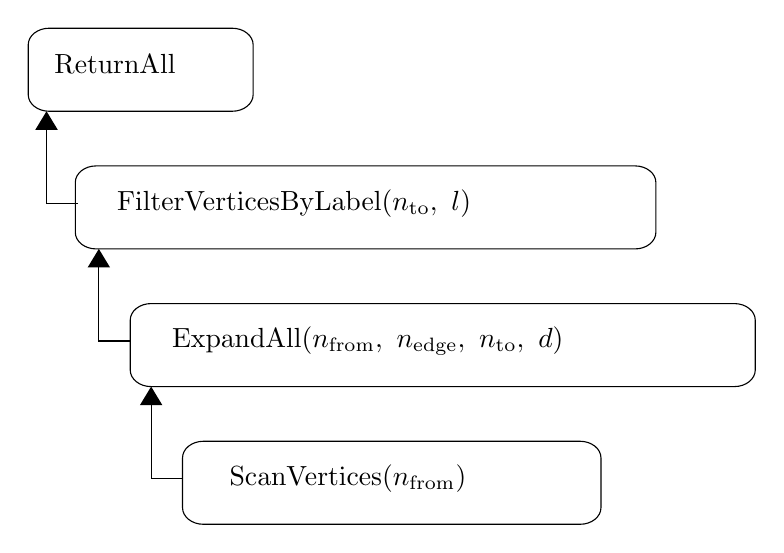
\begin{tikzpicture}[x=0.75pt,y=0.75pt,yscale=-1,xscale=1.26]
%uncomment if require: \path (0,300); %set diagram left start at 0, and has height of 300

%Rounded Rect [id:dp9370573454267987] 
\draw   (111,41) .. controls (111,36.58) and (114.58,33) .. (119,33) -- (189,33) .. controls (193.42,33) and (197,36.58) .. (197,41) -- (197,65) .. controls (197,69.42) and (193.42,73) .. (189,73) -- (119,73) .. controls (114.58,73) and (111,69.42) .. (111,65) -- cycle ;

%Rounded Rect [id:dp8665691991968861] 
\draw   (150,173.66) .. controls (150,169.24) and (153.58,165.66) .. (158,165.66) -- (381,165.66) .. controls (385.42,165.66) and (389,169.24) .. (389,173.66) -- (389,197.66) .. controls (389,202.08) and (385.42,205.66) .. (381,205.66) -- (158,205.66) .. controls (153.58,205.66) and (150,202.08) .. (150,197.66) -- cycle ;

%Rounded Rect [id:dp756749227156685] 
\draw   (170,240) .. controls (170,235.58) and (173.58,232) .. (178,232) -- (322,232) .. controls (326.42,232) and (330,235.58) .. (330,240) -- (330,264) .. controls (330,268.42) and (326.42,272) .. (322,272) -- (178,272) .. controls (173.58,272) and (170,268.42) .. (170,264) -- cycle ;

%Rounded Rect [id:dp9307818066691674] 
\draw   (129,107.33) .. controls (129,102.91) and (132.58,99.33) .. (137,99.33) -- (343,99.33) .. controls (347.42,99.33) and (351,102.91) .. (351,107.33) -- (351,131.33) .. controls (351,135.75) and (347.42,139.33) .. (343,139.33) -- (137,139.33) .. controls (132.58,139.33) and (129,135.75) .. (129,131.33) -- cycle ;

%Straight Lines [id:da678799978902756] 
\draw    (170,250) -- (158,250) -- (158,208.66) ;
\draw [shift={(158,205.66)}, rotate = 90] [fill={rgb, 255:red, 0; green, 0; blue, 0 }  ][line width=0.08]  [draw opacity=0] (8.93,-4.29) -- (0,0) -- (8.93,4.29) -- cycle    ;
%Straight Lines [id:da7443050345811884] 
\draw    (150,183.67) -- (138,183.67) -- (138,142.33) ;
\draw [shift={(138,139.33)}, rotate = 90] [fill={rgb, 255:red, 0; green, 0; blue, 0 }  ][line width=0.08]  [draw opacity=0] (8.93,-4.29) -- (0,0) -- (8.93,4.29) -- cycle    ;
%Straight Lines [id:da9837753990422333] 
\draw    (130,117.34) -- (118,117.34) -- (118,76) ;
\draw [shift={(118,73)}, rotate = 90] [fill={rgb, 255:red, 0; green, 0; blue, 0 }  ][line width=0.08]  [draw opacity=0] (8.93,-4.29) -- (0,0) -- (8.93,4.29) -- cycle    ;

% Text Node
\draw (120,44.5) node [anchor=north west][inner sep=0.75pt]   [align=left] {ReturnAll};
% Text Node
\draw (144,109.33) node [anchor=north west][inner sep=0.75pt]   [align=left] {FilterVerticesByLabel($\displaystyle n_{\text{to}} ,\ l)$};
% Text Node
\draw (165,175.66) node [anchor=north west][inner sep=0.75pt]   [align=left] {ExpandAll($\displaystyle n_{\text{from}} ,\ n_{\text{edge}} ,\ n_{\text{to}} ,\ d)$};
% Text Node
\draw (187,242) node [anchor=north west][inner sep=0.75pt]   [align=left] {ScanVertices($\displaystyle n_{\text{from}})$};


\end{tikzpicture}

  \caption{An example execution plan}
  \label{fig:example-execution-plan}
\end{figure}

\begin{definition}
  \textbf{An execution plan} is a chain of operations. For example consider Figure~\ref{fig:example-execution-plan}. The direction of arrows shows the order of operations and the flow of intermidiate tables.

  The node of an operation in the plan may or may not have a child depending on whether the operation takes an input table or not. The operation nodes that do not have children are called \textbf{leaf operations}. For now, we have only one leaf operation which is \texttt{ScanVertices}.
\end{definition}

\begin{definition}
  Using the operation evaluation function from the previous section, we can define \textbf{the execution plan evaluation function} $[\cdot]_G$ as follows:
  \begin{itemize}
    \item If the root node of a plan is a leaf operation then the evaluation function is just the evaluation function of the operation.
    \item If the root node of a plan is not a leaf operation then the evaluation function first evaluates the subplan of the child node and then feeds the resulting table to the evaluation function of the operation.

    For example, if the root node of the plan $p$ is $\texttt{ReturnAll}$ and the subplan is $p'$ then:
    $$ [p]_G = [\texttt{ReturnAll}]_G ([p']_G) $$
  \end{itemize}
\end{definition}

Note that this evaluation function is partial because the operation evalution function, used internally, is partial too. Generally, it means that the plan is ill-formed and doesn't really make a lot of sense.

\begin{definition}
  In the same way we defined the evaluation of execution plans, we can define \textbf{the type of an execution plan}. It is defined recursively on the structure of the plan and on each step we transform the type of the subplan the way described in the type axiom for the root operation.
  
  For example, if the root node of the plan $p$ is $\texttt{ReturnAll}$ and the subplan is $p'$ then:
    $$ T(p) = T(p') \mid_E $$
\end{definition}


\begin{definition}
  In a similar manner, we define \textbf{the well-formedness of a plan}. A plan is well-formed if the inputs to each operation satisfy the well-formedness conditions described in the operation definition but instead of using the type of the input table we use the type of the subplan, we have just defined.
\end{definition}

\begin{theorem}
  If $p$ is a well-formed plan then $[p]_G$ is defined.
\end{theorem}
\begin{proof}
  By straightforward induction on the structure of the plan and the well-formedness axioms for the operations.
\end{proof}

With this theorem we can easily show that the evaluation of a particular plan succeeds by simply looking at its structure.

We may now state an important connection between the type of a plan and the type of the resulting table. Unsurprisingly, they turn out to be equal.

\begin{theorem}
  If $p$ is a well-formed plan and $[p]_G$ is defined then
  $$T(p) = T([p]_G)$$
\end{theorem}
\begin{proof}
  By straightforward induction on the structure of the plan and the type axioms for the operations.
\end{proof}

This theorem means that we can easily find out the type of the resulting table without the need to evaluate the plan.

\subsection{The translation from queries to execution plans}

In this section we describe the translation algorithms from queries to execution plans that Neo4j and RedisGraph use to evaluate the queries.

We want to show that the translation is correct in the sense that the evaluation of the resulting execution plan, according to the specification of the execution plan, satisfies the specification of GQL.

\todo{the picture that explains everything}

% TODO: Show the scheme that explains what the correctness is.

\subsubsection{Neo4j}

The idea of this translation algorithm is to translate each edge pattern in a path pattern into the \texttt{Expand} operation, possibly adding instances of \texttt{FilterByLabel} to account for the labels in the vertex and edge patterns.

\begin{figure}
  

\tikzset{every picture/.style={line width=0.75pt}} %set default line width to 0.75pt        

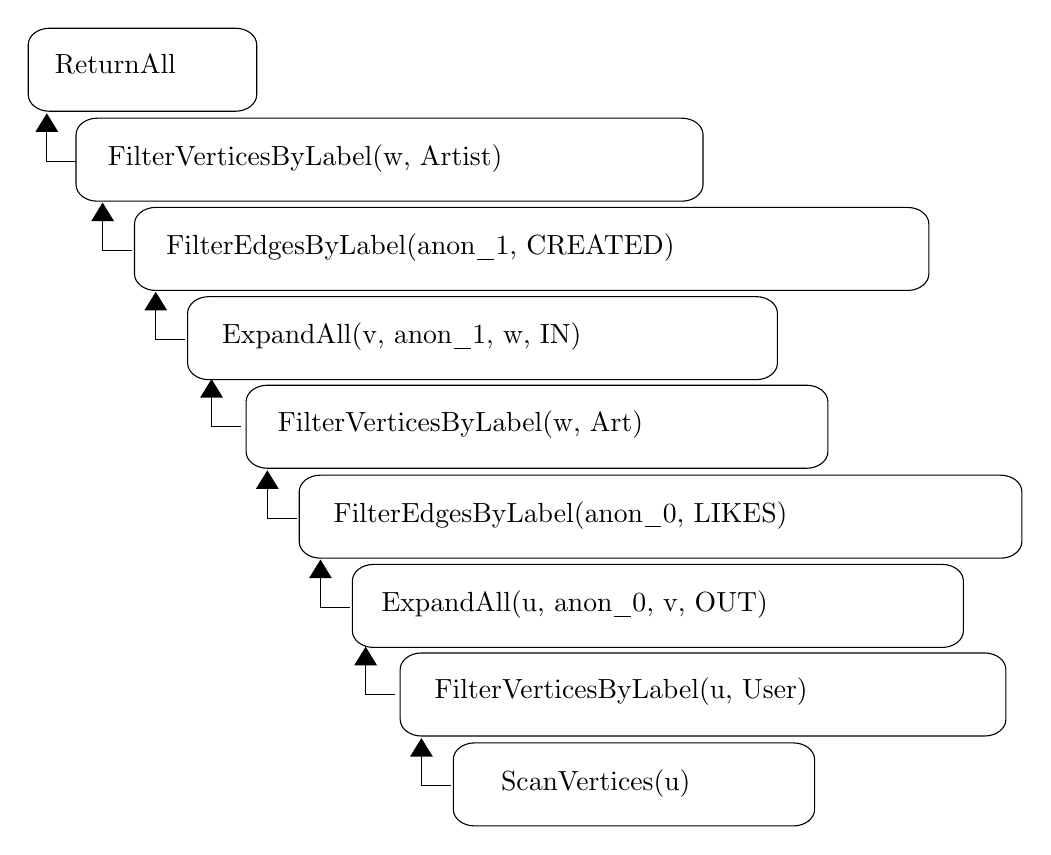
\begin{tikzpicture}[x=0.75pt,y=0.75pt,yscale=-1,xscale=1.28]
%uncomment if require: \path (0,531); %set diagram left start at 0, and has height of 531

%Rounded Rect [id:dp9370573454267987] 
\draw   (111,40) .. controls (111,35.58) and (114.58,32) .. (119,32) -- (189,32) .. controls (193.42,32) and (197,35.58) .. (197,40) -- (197,64) .. controls (197,68.42) and (193.42,72) .. (189,72) -- (119,72) .. controls (114.58,72) and (111,68.42) .. (111,64) -- cycle ;

%Rounded Rect [id:dp25448347116033077] 
\draw   (129,83.33) .. controls (129,78.91) and (132.58,75.33) .. (137,75.33) -- (357,75.33) .. controls (361.42,75.33) and (365,78.91) .. (365,83.33) -- (365,107.33) .. controls (365,111.75) and (361.42,115.33) .. (357,115.33) -- (137,115.33) .. controls (132.58,115.33) and (129,111.75) .. (129,107.33) -- cycle ;
%Straight Lines [id:da9837753990422333] 
\draw    (129,96) -- (118,96) -- (118,76) ;
\draw [shift={(118,73)}, rotate = 90] [fill={rgb, 255:red, 0; green, 0; blue, 0 }  ][line width=0.08]  [draw opacity=0] (8.93,-4.29) -- (0,0) -- (8.93,4.29) -- cycle    ;
%Rounded Rect [id:dp7780441432348261] 
\draw   (151,126.33) .. controls (151,121.91) and (154.58,118.33) .. (159,118.33) -- (442,118.33) .. controls (446.42,118.33) and (450,121.91) .. (450,126.33) -- (450,150.33) .. controls (450,154.75) and (446.42,158.33) .. (442,158.33) -- (159,158.33) .. controls (154.58,158.33) and (151,154.75) .. (151,150.33) -- cycle ;
%Straight Lines [id:da014130696077634952] 
\draw    (150,139) -- (139,139) -- (139,119) ;
\draw [shift={(139,116)}, rotate = 90] [fill={rgb, 255:red, 0; green, 0; blue, 0 }  ][line width=0.08]  [draw opacity=0] (8.93,-4.29) -- (0,0) -- (8.93,4.29) -- cycle    ;
%Rounded Rect [id:dp6856967461478435] 
\draw   (171,169.33) .. controls (171,164.91) and (174.58,161.33) .. (179,161.33) -- (395 - 10,161.33) .. controls (399.42 - 10,161.33) and (403 - 10,164.91) .. (403 - 10,169.33) -- (403 - 10,193.33) .. controls (403 - 10,197.75) and (399.42 - 10,201.33) .. (395 - 10,201.33) -- (179,201.33) .. controls (174.58,201.33) and (171,197.75) .. (171,193.33) -- cycle ;
%Straight Lines [id:da3265514824492094] 
\draw    (170,182) -- (159,182) -- (159,162) ;
\draw [shift={(159,159)}, rotate = 90] [fill={rgb, 255:red, 0; green, 0; blue, 0 }  ][line width=0.08]  [draw opacity=0] (8.93,-4.29) -- (0,0) -- (8.93,4.29) -- cycle    ;
%Rounded Rect [id:dp8312842736537362] 
\draw   (193,212) .. controls (193,207.58) and (196.58,204) .. (201,204) -- (404,204) .. controls (408.42,204) and (412,207.58) .. (412,212) -- (412,236) .. controls (412,240.42) and (408.42,244) .. (404,244) -- (201,244) .. controls (196.58,244) and (193,240.42) .. (193,236) -- cycle ;
%Straight Lines [id:da3212722162870766] 
\draw    (191,224) -- (180,224) -- (180,204) ;
\draw [shift={(180,201)}, rotate = 90] [fill={rgb, 255:red, 0; green, 0; blue, 0 }  ][line width=0.08]  [draw opacity=0] (8.93,-4.29) -- (0,0) -- (8.93,4.29) -- cycle    ;
%Rounded Rect [id:dp21603275316052373] 
\draw   (213,255.33) .. controls (213,250.91) and (216.58,247.33) .. (221,247.33) -- (477,247.33) .. controls (481.42,247.33) and (485,250.91) .. (485,255.33) -- (485,279.33) .. controls (485,283.75) and (481.42,287.33) .. (477,287.33) -- (221,287.33) .. controls (216.58,287.33) and (213,283.75) .. (213,279.33) -- cycle ;
%Straight Lines [id:da5794885178740662] 
\draw    (212,268) -- (201,268) -- (201,248) ;
\draw [shift={(201,245)}, rotate = 90] [fill={rgb, 255:red, 0; green, 0; blue, 0 }  ][line width=0.08]  [draw opacity=0] (8.93,-4.29) -- (0,0) -- (8.93,4.29) -- cycle    ;
%Rounded Rect [id:dp4438884800021361] 
\draw   (233,298.33) .. controls (233,293.91) and (236.58,290.33) .. (241,290.33) -- (455,290.33) .. controls (459.42,290.33) and (463,293.91) .. (463,298.33) -- (463,322.33) .. controls (463,326.75) and (459.42,330.33) .. (455,330.33) -- (241,330.33) .. controls (236.58,330.33) and (233,326.75) .. (233,322.33) -- cycle ;
%Straight Lines [id:da8951131696919742] 
\draw    (232,311) -- (221,311) -- (221,291) ;
\draw [shift={(221,288)}, rotate = 90] [fill={rgb, 255:red, 0; green, 0; blue, 0 }  ][line width=0.08]  [draw opacity=0] (8.93,-4.29) -- (0,0) -- (8.93,4.29) -- cycle    ;
%Rounded Rect [id:dp6556013644458546] 
\draw   (251,341) .. controls (251,336.58) and (254.58,333) .. (259,333) -- (471,333) .. controls (475.42,333) and (479,336.58) .. (479,341) -- (479,365) .. controls (479,369.42) and (475.42,373) .. (471,373) -- (259,373) .. controls (254.58,373) and (251,369.42) .. (251,365) -- cycle ;
%Straight Lines [id:da4631977993157814] 
\draw    (249,353) -- (238,353) -- (238,333) ;
\draw [shift={(238,330)}, rotate = 90] [fill={rgb, 255:red, 0; green, 0; blue, 0 }  ][line width=0.08]  [draw opacity=0] (8.93,-4.29) -- (0,0) -- (8.93,4.29) -- cycle    ;
%Rounded Rect [id:dp8868145464168437] 
\draw   (271,384.33) .. controls (271,379.91) and (274.58,376.33) .. (279,376.33) -- (399,376.33) .. controls (403.42,376.33) and (407,379.91) .. (407,384.33) -- (407,408.33) .. controls (407,412.75) and (403.42,416.33) .. (399,416.33) -- (279,416.33) .. controls (274.58,416.33) and (271,412.75) .. (271,408.33) -- cycle ;
%Straight Lines [id:da6792309496243043] 
\draw    (270,397) -- (259,397) -- (259,377) ;
\draw [shift={(259,374)}, rotate = 90] [fill={rgb, 255:red, 0; green, 0; blue, 0 }  ][line width=0.08]  [draw opacity=0] (8.93,-4.29) -- (0,0) -- (8.93,4.29) -- cycle    ;

% Text Node
\draw (120,43.5) node [anchor=north west][inner sep=0.75pt]   [align=left] {ReturnAll};
% Text Node
\draw (140,86.83) node [anchor=north west][inner sep=0.75pt]   [align=left] {FilterVerticesByLabel(w, Artist)};
% Text Node
\draw (162,129.83) node [anchor=north west][inner sep=0.75pt]   [align=left] {FilterEdgesByLabel(anon\_1, CREATED)};
% Text Node
\draw (183,172.83) node [anchor=north west][inner sep=0.75pt]   [align=left] {ExpandAll(v, anon\_1, w, IN)};
% Text Node
\draw (204,214.83) node [anchor=north west][inner sep=0.75pt]   [align=left] {FilterVerticesByLabel(w, Art)};
% Text Node
\draw (225,258.83) node [anchor=north west][inner sep=0.75pt]   [align=left] {FilterEdgesByLabel(anon\_0, LIKES)};
% Text Node
\draw (243,301.83) node [anchor=north west][inner sep=0.75pt]   [align=left] {ExpandAll(u, anon\_0, v, OUT)};
% Text Node
\draw (263,343.83) node [anchor=north west][inner sep=0.75pt]   [align=left] {FilterVerticesByLabel(u, User)};
% Text Node
\draw (288,387.83) node [anchor=north west][inner sep=0.75pt]   [align=left] {ScanVertices(u)};


\end{tikzpicture}

  \caption{The Neo4j execution plan for the example path pattern}
  \label{fig:neo4j-execution-plan}
\end{figure}

For example, we have the following path pattern:
\begin{verbatim}
  (u:User)-[:LIKES]->(v:Art)<-[:CREATED]-(w:Artist)
\end{verbatim}
Suppose that after normalization the first edge pattern got the name \texttt{anon\_0} and the second one got the name \texttt{anon\_1}. Then the translation algorithm produces the execution plan on Figure~\ref{fig:neo4j-execution-plan}.

\begin{figure}
  

\tikzset{every picture/.style={line width=0.75pt}} %set default line width to 0.75pt        

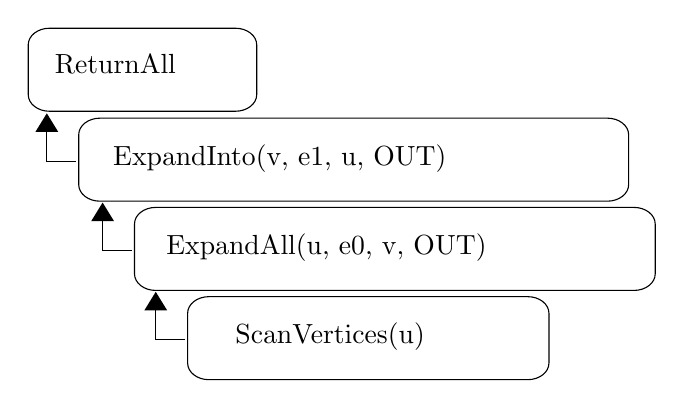
\begin{tikzpicture}[x=0.75pt,y=0.75pt,yscale=-1,xscale=1.28]
%uncomment if require: \path (0,531); %set diagram left start at 0, and has height of 531

%Rounded Rect [id:dp9370573454267987] 
\draw   (111,40) .. controls (111,35.58) and (114.58,32) .. (119,32) -- (189,32) .. controls (193.42,32) and (197,35.58) .. (197,40) -- (197,64) .. controls (197,68.42) and (193.42,72) .. (189,72) -- (119,72) .. controls (114.58,72) and (111,68.42) .. (111,64) -- cycle ;

%Rounded Rect [id:dp6856967461478435] 
\draw   (130,83.33) .. controls (130,78.91) and (133.58,75.33) .. (138,75.33) -- (329,75.33) .. controls (333.42,75.33) and (337,78.91) .. (337,83.33) -- (337,107.33) .. controls (337,111.75) and (333.42,115.33) .. (329,115.33) -- (138,115.33) .. controls (133.58,115.33) and (130,111.75) .. (130,107.33) -- cycle ;
%Straight Lines [id:da3265514824492094] 
\draw    (129,96) -- (118,96) -- (118,76) ;
\draw [shift={(118,73)}, rotate = 90] [fill={rgb, 255:red, 0; green, 0; blue, 0 }  ][line width=0.08]  [draw opacity=0] (8.93,-4.29) -- (0,0) -- (8.93,4.29) -- cycle    ;
%Rounded Rect [id:dp4438884800021361] 
\draw   (151,126.33) .. controls (151,121.91) and (154.58,118.33) .. (159,118.33) -- (339,118.33) .. controls (343.42,118.33) and (347,121.91) .. (347,126.33) -- (347,150.33) .. controls (347,154.75) and (343.42,158.33) .. (339,158.33) -- (159,158.33) .. controls (154.58,158.33) and (151,154.75) .. (151,150.33) -- cycle ;
%Straight Lines [id:da8951131696919742] 
\draw    (150,139) -- (139,139) -- (139,119) ;
\draw [shift={(139,116)}, rotate = 90] [fill={rgb, 255:red, 0; green, 0; blue, 0 }  ][line width=0.08]  [draw opacity=0] (8.93,-4.29) -- (0,0) -- (8.93,4.29) -- cycle    ;
%Rounded Rect [id:dp8868145464168437] 
\draw   (171,169.33) .. controls (171,164.91) and (174.58,161.33) .. (179,161.33) -- (299,161.33) .. controls (303.42,161.33) and (307,164.91) .. (307,169.33) -- (307,193.33) .. controls (307,197.75) and (303.42,201.33) .. (299,201.33) -- (179,201.33) .. controls (174.58,201.33) and (171,197.75) .. (171,193.33) -- cycle ;
%Straight Lines [id:da6792309496243043] 
\draw    (170,182) -- (159,182) -- (159,162) ;
\draw [shift={(159,159)}, rotate = 90] [fill={rgb, 255:red, 0; green, 0; blue, 0 }  ][line width=0.08]  [draw opacity=0] (8.93,-4.29) -- (0,0) -- (8.93,4.29) -- cycle    ;

% Text Node
\draw (120,43.5) node [anchor=north west][inner sep=0.75pt]   [align=left] {ReturnAll};
% Text Node
\draw (142,86.83) node [anchor=north west][inner sep=0.75pt]   [align=left] {ExpandInto(v, e1, u, OUT)};
% Text Node
\draw (162,129.83) node [anchor=north west][inner sep=0.75pt]   [align=left] {ExpandAll(u, e0, v, OUT)};
% Text Node
\draw (188,172.83) node [anchor=north west][inner sep=0.75pt]   [align=left] {ScanVertices(u)};


\end{tikzpicture}

  \caption{The Neo4j execution plan for the example cyclic path pattern}
  \label{fig:neo4j-execution-plan-cyclic}
\end{figure}

Is is also worth to consider the case of cyclic path patterns. For example, we have the following path pattern:
% which specifies directed cycles with two edges:
\begin{verbatim}
  (u)-[e0]->(v)-[e1]->(u)
\end{verbatim}
To the point where we process the second edge pattern, both \texttt{u} and \texttt{v} are already in the context. That is why we use \texttt{ExpandInto} instead of \texttt{ExpandAll} and get the execution plan on Figure~\ref{fig:neo4j-execution-plan-cyclic}.

\begin{definition}
  We can now precisely define \textbf{the auxilliary translation algorithm} from path patterns to execution plans. Let's denote the auxilliary plan for a path pattern $\pi$ by $P'(\pi)$. The algorithm is defined as follows:
  \begin{itemize}
    \item If the path pattern is of the form $\patternstart{\pi_v}$ where $\pi_v$ is a vertex pattern that has name $n$ and label $l$ then the execution plan for $(\pi_v)$ is \texttt{ScanVertices(n)} followed by \texttt{FilterVerticesByLabel(n, l)}. If $l$ is not specified then the execution plan is just \texttt{ScanVertices(n)}.

    \item If the path pattern is of the form $\patternhop{\pi}{\pi_e}{\pi_v}$ where $\pi$ is a path pattern where the name of the last vertex pattern is $n_u$; $\pi_e$ is an edge pattern that has name $n_e$, direction $d$ and label $l_e$, and $\pi_v$ is a vertex pattern that has name $n_v$ and label $l_v$; then the execution plan for $\patternhop{\pi}{\pi_e}{\pi_v}$ is \texttt{Expand}($m$, $n_u$, $n_e$, $n_v$) followed by \texttt{FilterEdgesByLabel}($n_e$, $l_e$) and \texttt{FilterVerticesByLabel}($n_v$, $l_v$). 
    If any of the labels is not specified, the corresponding filtering operation is not included. The mode $m$ of the \texttt{Expand} operation is determined based on whether $n_v$ is already present or not. This can be checked by looking at $T_F(\pi)$, the full type of the pattern.
  \end{itemize} 
\end{definition}

\begin{definition}
  \textbf{The translation algorithm} itself just runs the auxilliary algorithm $P'$ and appends the \texttt{ReturnAll} operation to the plan.
  Let's denote the plan for a path pattern $\pi$ by $P(\pi)$.
\end{definition}

We can now show lots of important properties using the machinery we developed earlier.

\begin{lemma}
  \label{lem:neo4j-translation-type}
  If $\pi$ is well-formed then
  $$T(P'(\pi)) = T_F(\pi)$$
  In other words, the type of the auxilliary plan is the full type of the path pattern (remember, $F$ stands for \textit{full} matching mode)
\end{lemma}
\begin{proof}
  By straightforward induction on the structure of the pattern.
\end{proof}

That is, the \texttt{Expand} operation doesn't differentiate between implicit and explicit names which means that all the names are present in the resulting binding table. That is why the last lemma is stated using the full matching mode. However, after the \texttt{ReturnAll} operation, only the names that were explicitly specified in the path pattern are left in the result. This is reflected in the following theorem.

\begin{theorem}
  \label{thm:neo4j-translation-type}
  If $\pi$ is well-formed then
  $$T(P(\pi)) = T_E(\pi)$$
\end{theorem}
\begin{proof}
  $ T(P(\pi)) = T(P'(\pi))|_E = T_F(\pi)|_E = T_E(\pi) $
\end{proof}

\begin{lemma} If $\pi$ is well-formed then
  $$[P'(\pi)]_G = \{ r \mid \exists p : (G, p, r) \models_F \pi \}$$
\end{lemma}
\begin{proof}
  By straightforward induction on the structure of the pattern.
\end{proof}

We again use the full matching mode because all the names are necessary for this translation algorithm to compute the result. As we already mentioned, we could have weaken the pattern-matching predicate to work only with explicit names leaving the behavior for implicit names unspecified. However, this would make it impossible to prove the following theorem because the \texttt{Expand} operation would refer to and rely on the unspecified data which is from the standpoint of rigourous proofs is absolutely arbitrary.

\begin{theorem} If $\pi$ is well-formed then
  $$[P(\pi)]_G = \{ r \mid \exists p : (G, p, r) \models_E \pi \}$$
\end{theorem}
\begin{proof} From the specification of \texttt{ReturnAll} and the previous theorem we know:
  $$[P(\pi)]_G = \{ r|_E \mid r \in [P'(\pi)]_G \} = \{ r|_E \mid \exists p : (G, p, r) \models_F \pi \} $$
  So we need to prove that:
  $$ \{ r|_E \mid \exists p : (G, p, r) \models_F \pi \} = \{ r \mid \exists p : (G, p, r) \models_E \pi \} $$
  By the theorem~\ref{thm:matching-mode-narrow} we already know that if $(G, p, r) \models_F \pi$ then $(G, p, r |_E) \models_E \pi$. Moreover, by the theorem~\ref{thm:matching-mode-widen} we know that if $(G, p, r') \models_E \pi$ then there is $r$ such that $r' = r|_E$ and $(G, p, r) \models_F \pi$. So we can conclude that the equality holds.
\end{proof}

The last theorem is the most important one because it shows that the translation algorithm does exactly what we want from it: it finds all the paths that match the pattern and returns only the names that were explicitly specified in the pattern.

\begin{lemma}
  If $\pi$ is well-formed then $P'(\pi)$ is well-formed.
\end{lemma}
\begin{proof}
  By straightforward induction on the structure of the pattern and usage of the lemma~\ref{lem:neo4j-translation-type}.
\end{proof}

\begin{theorem}
  If $\pi$ is well-formed then $P(\pi)$ is well-formed.
\end{theorem}
\begin{proof}
  \texttt{ReturnAll} doesn't pose any new well-formedness restrictions.
\end{proof}

Let $q$ be a query and $\pi$ its path pattern. Let's define the query evaluation function as $[q]_G := [P(\pi)]_G$. We can now show that it satisfies the specification of GQL using the just proven theorems.

\subsubsection{RedisGraph}

\todo{...}

\subsection{The implementation of the execution plan operations}

Implementing almost all of the operations is pretty straightforward because they are simple enough. It is worth noting that we mostly aim to provide an implementation that just works. We are not trying to optimize the implementation for performance as it is out of the scope of this project.

However, one RedisGraph-specific operation is much more complex. Even though, we could implement it in a similar way as any other: making it just work, we decided that we want to capture the way RedisGraph implements it: using matrices. 

It has to translate a pattern slice into a complex matrix expression, evaluate the expression and iterate over the resulting matrix producing the resulting table. 

\todo{...}

\section{The mechanization in Coq}

In this section we describe the layout of Coq project and outline where the definitions and theorems are located.

\subsection{The project dependencies}

We use the following libraries:
\begin{itemize}
  \item \href{https://github.com/vafeiadis/hahn}{\texttt{hahn}} for a lot of convenient automation tactics;
  \item \href{http://perso.ens-lyon.fr/damien.pous/ra/}{\texttt{relational-algebra}} for the boolean matrices.
\end{itemize}

\subsection{The files structure}

We have the following files in the project. Each file depends only on the files that are listed before:
\begin{itemize}
  \item \texttt{Utils.v} contains some utility definitions and lemmas that are absent in the standard library;
  \item \texttt{RAUtils.v} contains some utility definitions and lemmas that are absent in the relational-algebra library;
  \item \texttt{Maps.v} contains the definitions of total and partial maps, which are then used to define records and their types, the update syntax and some lemmas about them;
  \item \texttt{PropertyGraph.v} contains the definition of the property graphs;
  \item \texttt{Cypher.v} contains the definition of the GQL abstract syntax, including names and path patterns;
  \item \texttt{BindingTable.v} contains the definitions of the values, types and binding tables;
  \item \texttt{Semantics.v} contains the specification of the GQL semantics, including matching modes and the pattern-matching predicate;
  \item \texttt{PatternE.v} contains the definitions of the pattern and path slices and the pattern-matching predicate for them;
  \item \texttt{ExecutionPlan.v} contains the specification of the execution plan;
  \item \texttt{Translation.v} contains the Neo4j-like translation algorithm and the proof of its correctness;
  \item \texttt{Translation2.v} contains the RedisGraph-like translation algorithm and the proof of its correctness;
  \item \texttt{TraverseOpImpl.v} contains the implementation of the \texttt{Traverse} operation and the proof of its correctness;
  \item \texttt{ExecutionPlanImpl.v} contains the implementation of all the other operations and the proof of their correctness.
\end{itemize}

\subsection{The used axioms}

This project only supposes \textit{the functional extensionality} axiom. It is used to prove the equalities between binding tables' records because records are defined as functions from names to values.

We don't apply, for example, \textit{the law of excluded middle} or any other axiom from classical logic which means that our proofs are fully constructive.

\todo{how we used modules and functors for specifications}
\todo{the mapping from definitions to files}

% У заключения нет номера главы
\section*{Conclusion and future work}

In summary, we aimed to write the specification of a subset of GQL and execution plans and show the correctness of the query translation for two reference databases, Neo4j and RedisGraph. We have completed all our subgoals:

\begin{itemize}
  \item We have mechanized the specification of the core subset of the GQL standard via abstract syntax and denotational semantics.
  \item We have mechanized the specification of the execution plan via denotational semantics.
  \item We have implement and prove the correctness of the translation of the queries for both reference databases.
  \item We have provided an example implementation of the execution plan evaluation including the implementation of the \texttt{Traverse} operation using matrices.
\end{itemize}

There are many directions in which this project can go. For example, we can continue by expanding the current subset of GQL or turn our code into an extensible framework to allow easier reasoning about graph query languages and their semantics.

\setmonofont[Mapping=tex-text]{CMU Typewriter Text}
% \pagenumbering{gobble}
% \bibliographystyle{plain}
% \bibliography{thesis}
\printbibliography
\end{document}
